\documentclass[ ../main.tex]{subfiles}
\providecommand{\mainx}{..}
\begin{document}
\section{Performance evaluation}
\label{performance-evaluation}
\begin{figure}
\label{fig3}
\centering
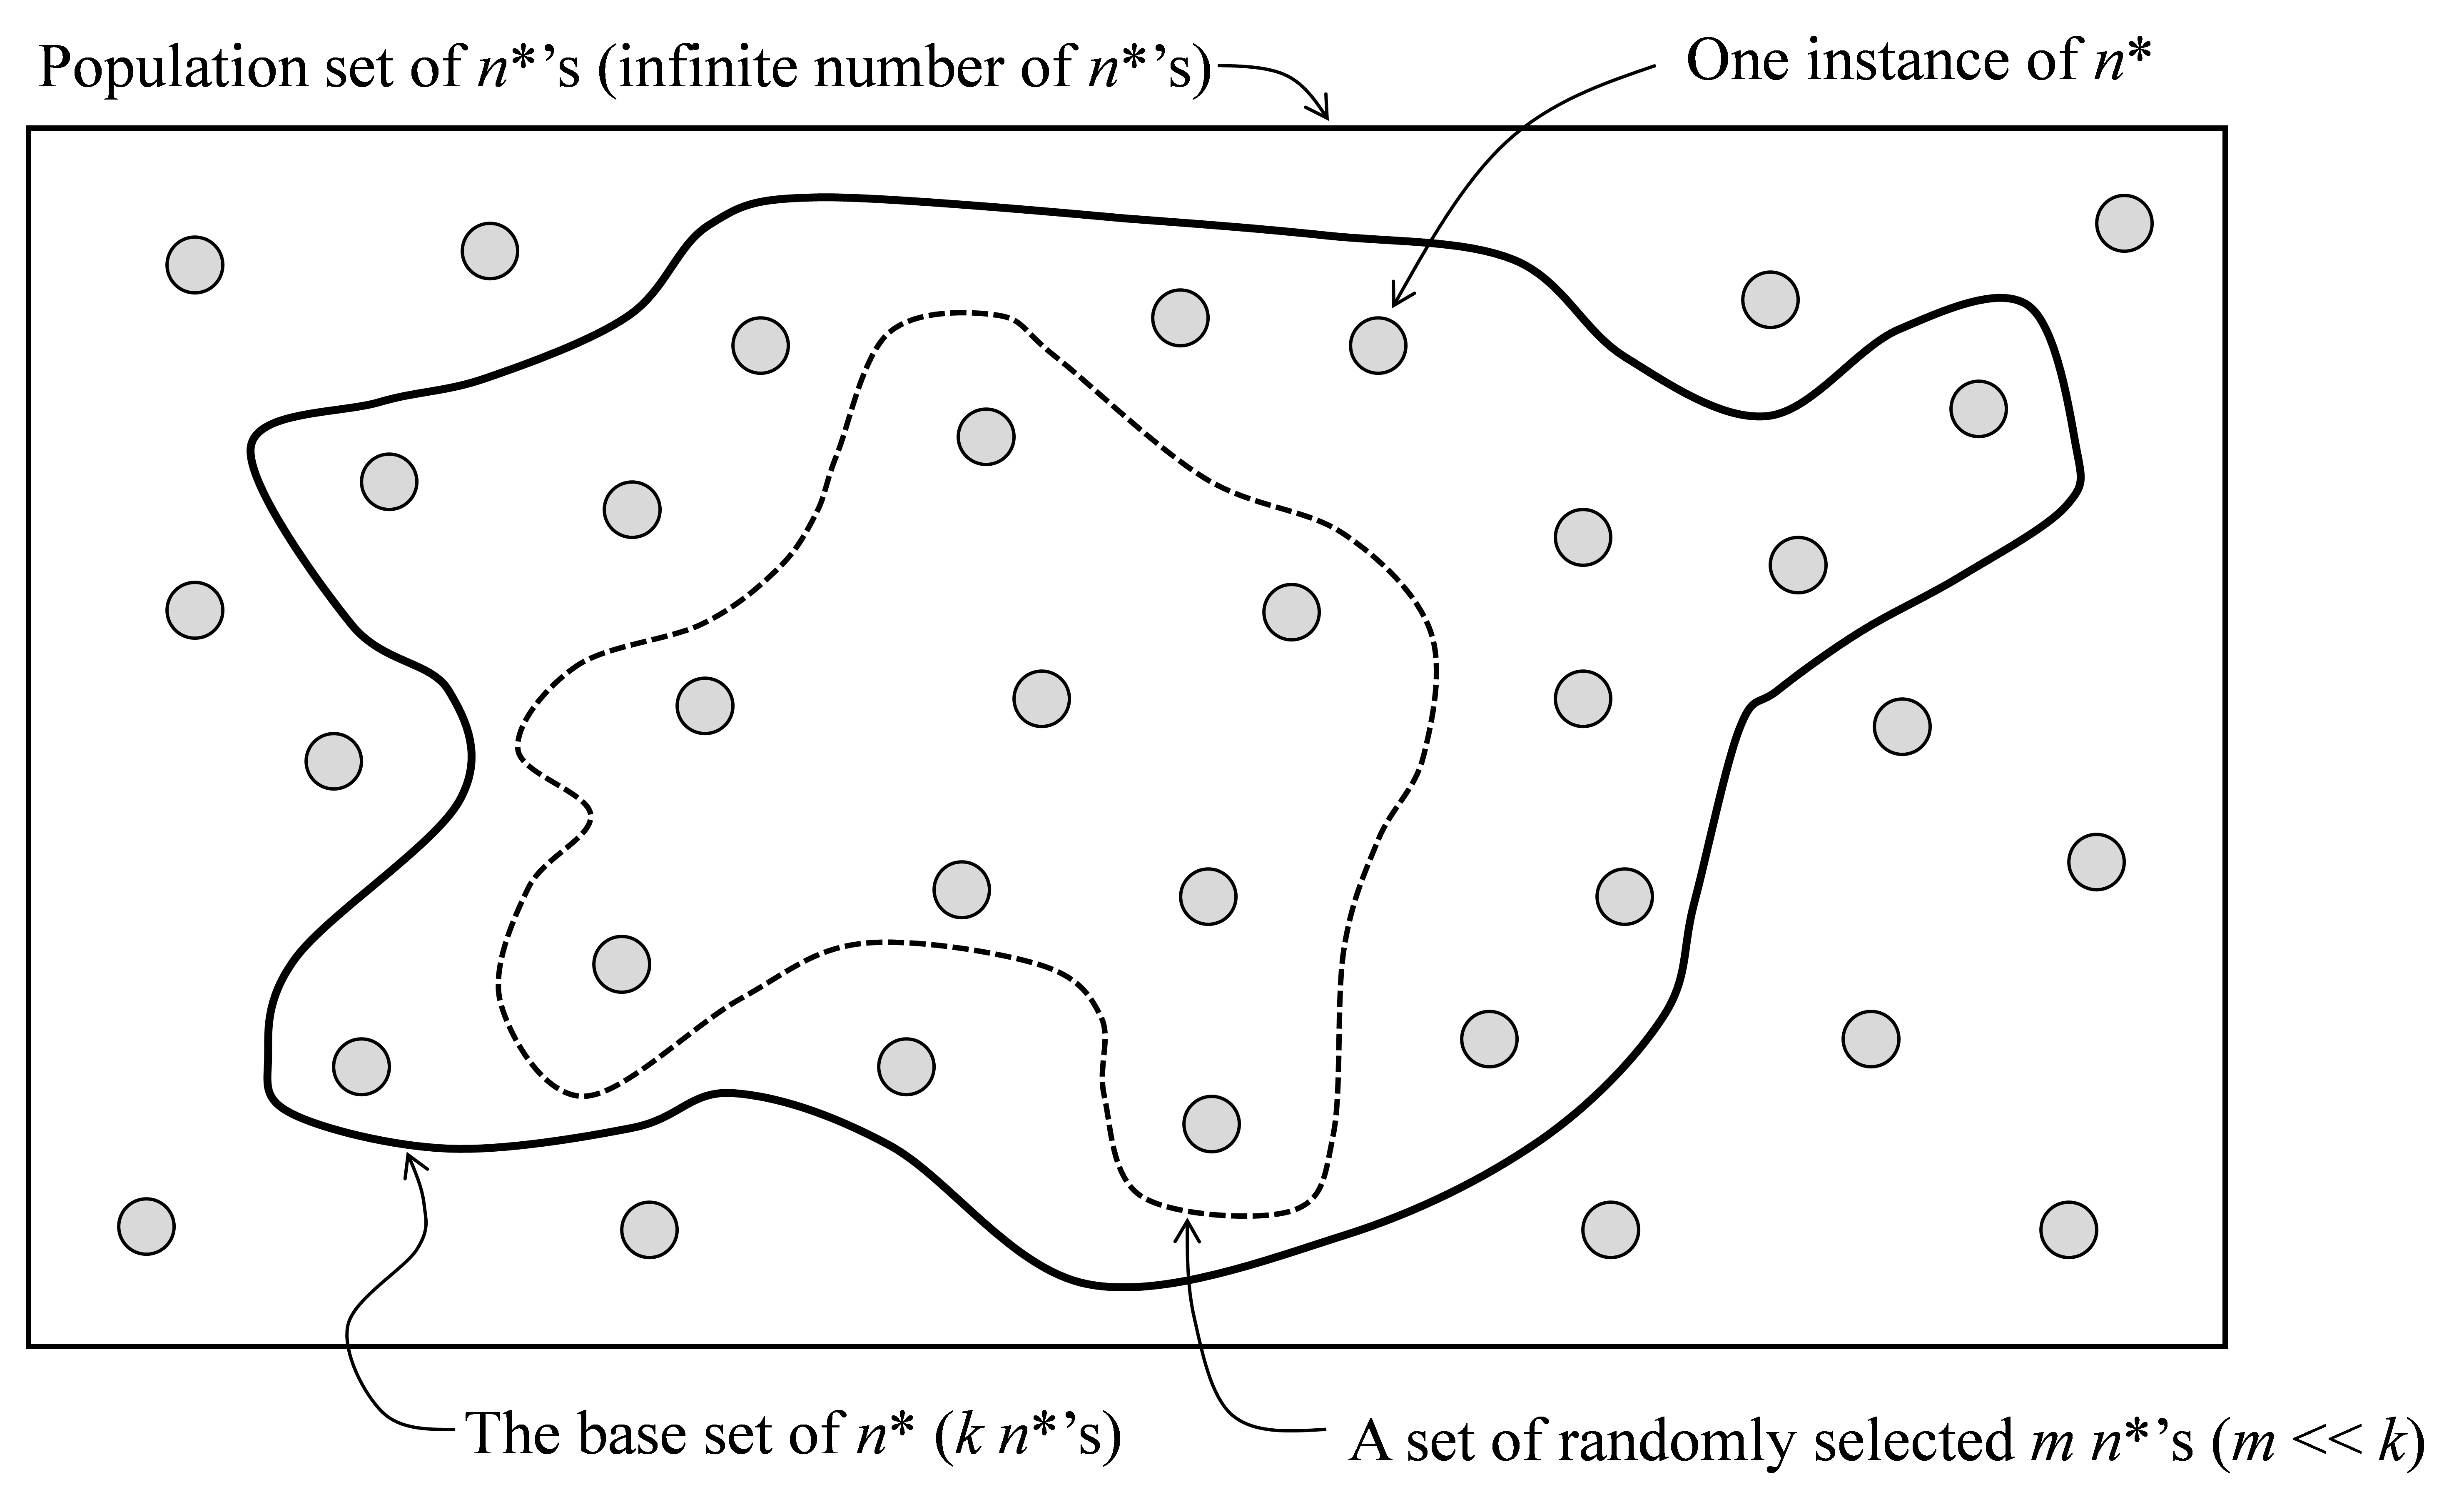
\includegraphics[width=0.9\textwidth]{images/fig3.png}
\caption{Bootstrapping of $m$ samples}
\end{figure}



We compared the performance of our bootstrap method for estimating $N^*$ using only $m$ samples with that of the ideal case (i.e., the one for representing the population set), using a large value
$k$, which will produce $N^*$ close to that for the infinite sample size. For that purpose, we compared the cumulative distribution functions of the 5th percentile (i.e., $\theta = 0.05$) for the population and empirical distributions.

\Cref{fig5a,fig5b,fig5c} show the population and empirical cumulative distribution functions from our experiments for the following configuration: $p^* = 0.30$, $\theta = 0.05$, $k = 5000$, and $s = 10000$ for $m = 50, 100$, and $250$, respectively. The experiments demonstrated the following observations. For a small sampling size ($m = 50$), the population and empirical sampling distributions are nothing alike. As $m$ (the bootstrap sampling size) increases, the population and empirical sampling distributions quickly converge to the same shape. After $m = 500$, no significant difference was observed between the two distributions.

\begin{figure}
\centering
\subfloat[$m = 50$\label{fig5c}]
{%
    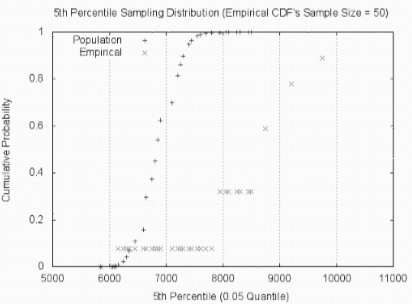
\includegraphics[width=0.3\textwidth]{images/fig5a.png}
}
\hfill
\subfloat[$m = 100$\label{fig5b}]
{%
    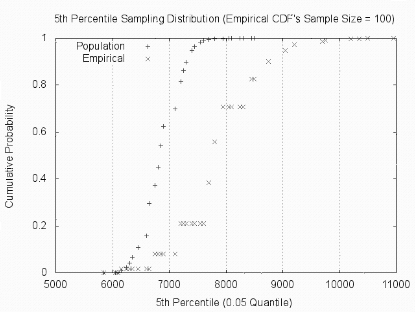
\includegraphics[width=0.3\textwidth]{images/fig5b.png}
}
\hfill
\subfloat[$m = 250$\label{fig5c}]
{%
    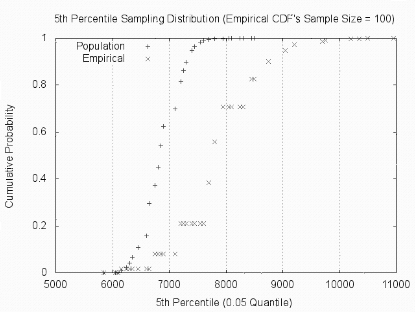
\includegraphics[width=0.3\textwidth]{images/fig5b.png}
}
\caption{The population and empirical cumulative distribution functions of the 5th percentile for bootstrap sample sizes $m = 50$, $100$, and $250$.}
\label{fig:pop_vs_emp_cdf}
\end{figure}

We studied the effect of $\theta$ to $N^*$ when we increased $\theta$ from $0.01$ to $0.50$. Our simulation experiments for the above analyses generated approximately $6$ GB of raw data, from which we made the following observations.

Figure 6 shows the $N^*$'s, as well as their lower and the upper $95\%$ thresholds, for different levels of the probability ($\theta = 0.01$ through $0.50$) an adversary achieves for an accuracy level of $p^* = 0.30$. The means between the bottom and ceiling of $95\%$ \CI (the crosshairs on the solid line) were calculated by taking the means of their sampling distribution.

We repeated the same analyses for the adversary accuracy of $45$ and $50\%$ (i.e., $p^* = 0.45$ and $0.50$). This is a scenario in which an adversary can correctly map $45$ and $50\%$ of what the adversary observed by a $5\%$ chance ($\theta = 0.05$), respectively.

\begin{figure}
\centering
\label{fig6}
\caption{$N^*$ for different levels of the probability for $\theta = 0.01$ through $0.50$ an adversary achieves for an adversary accuracy of $p^* = 0.30$.}
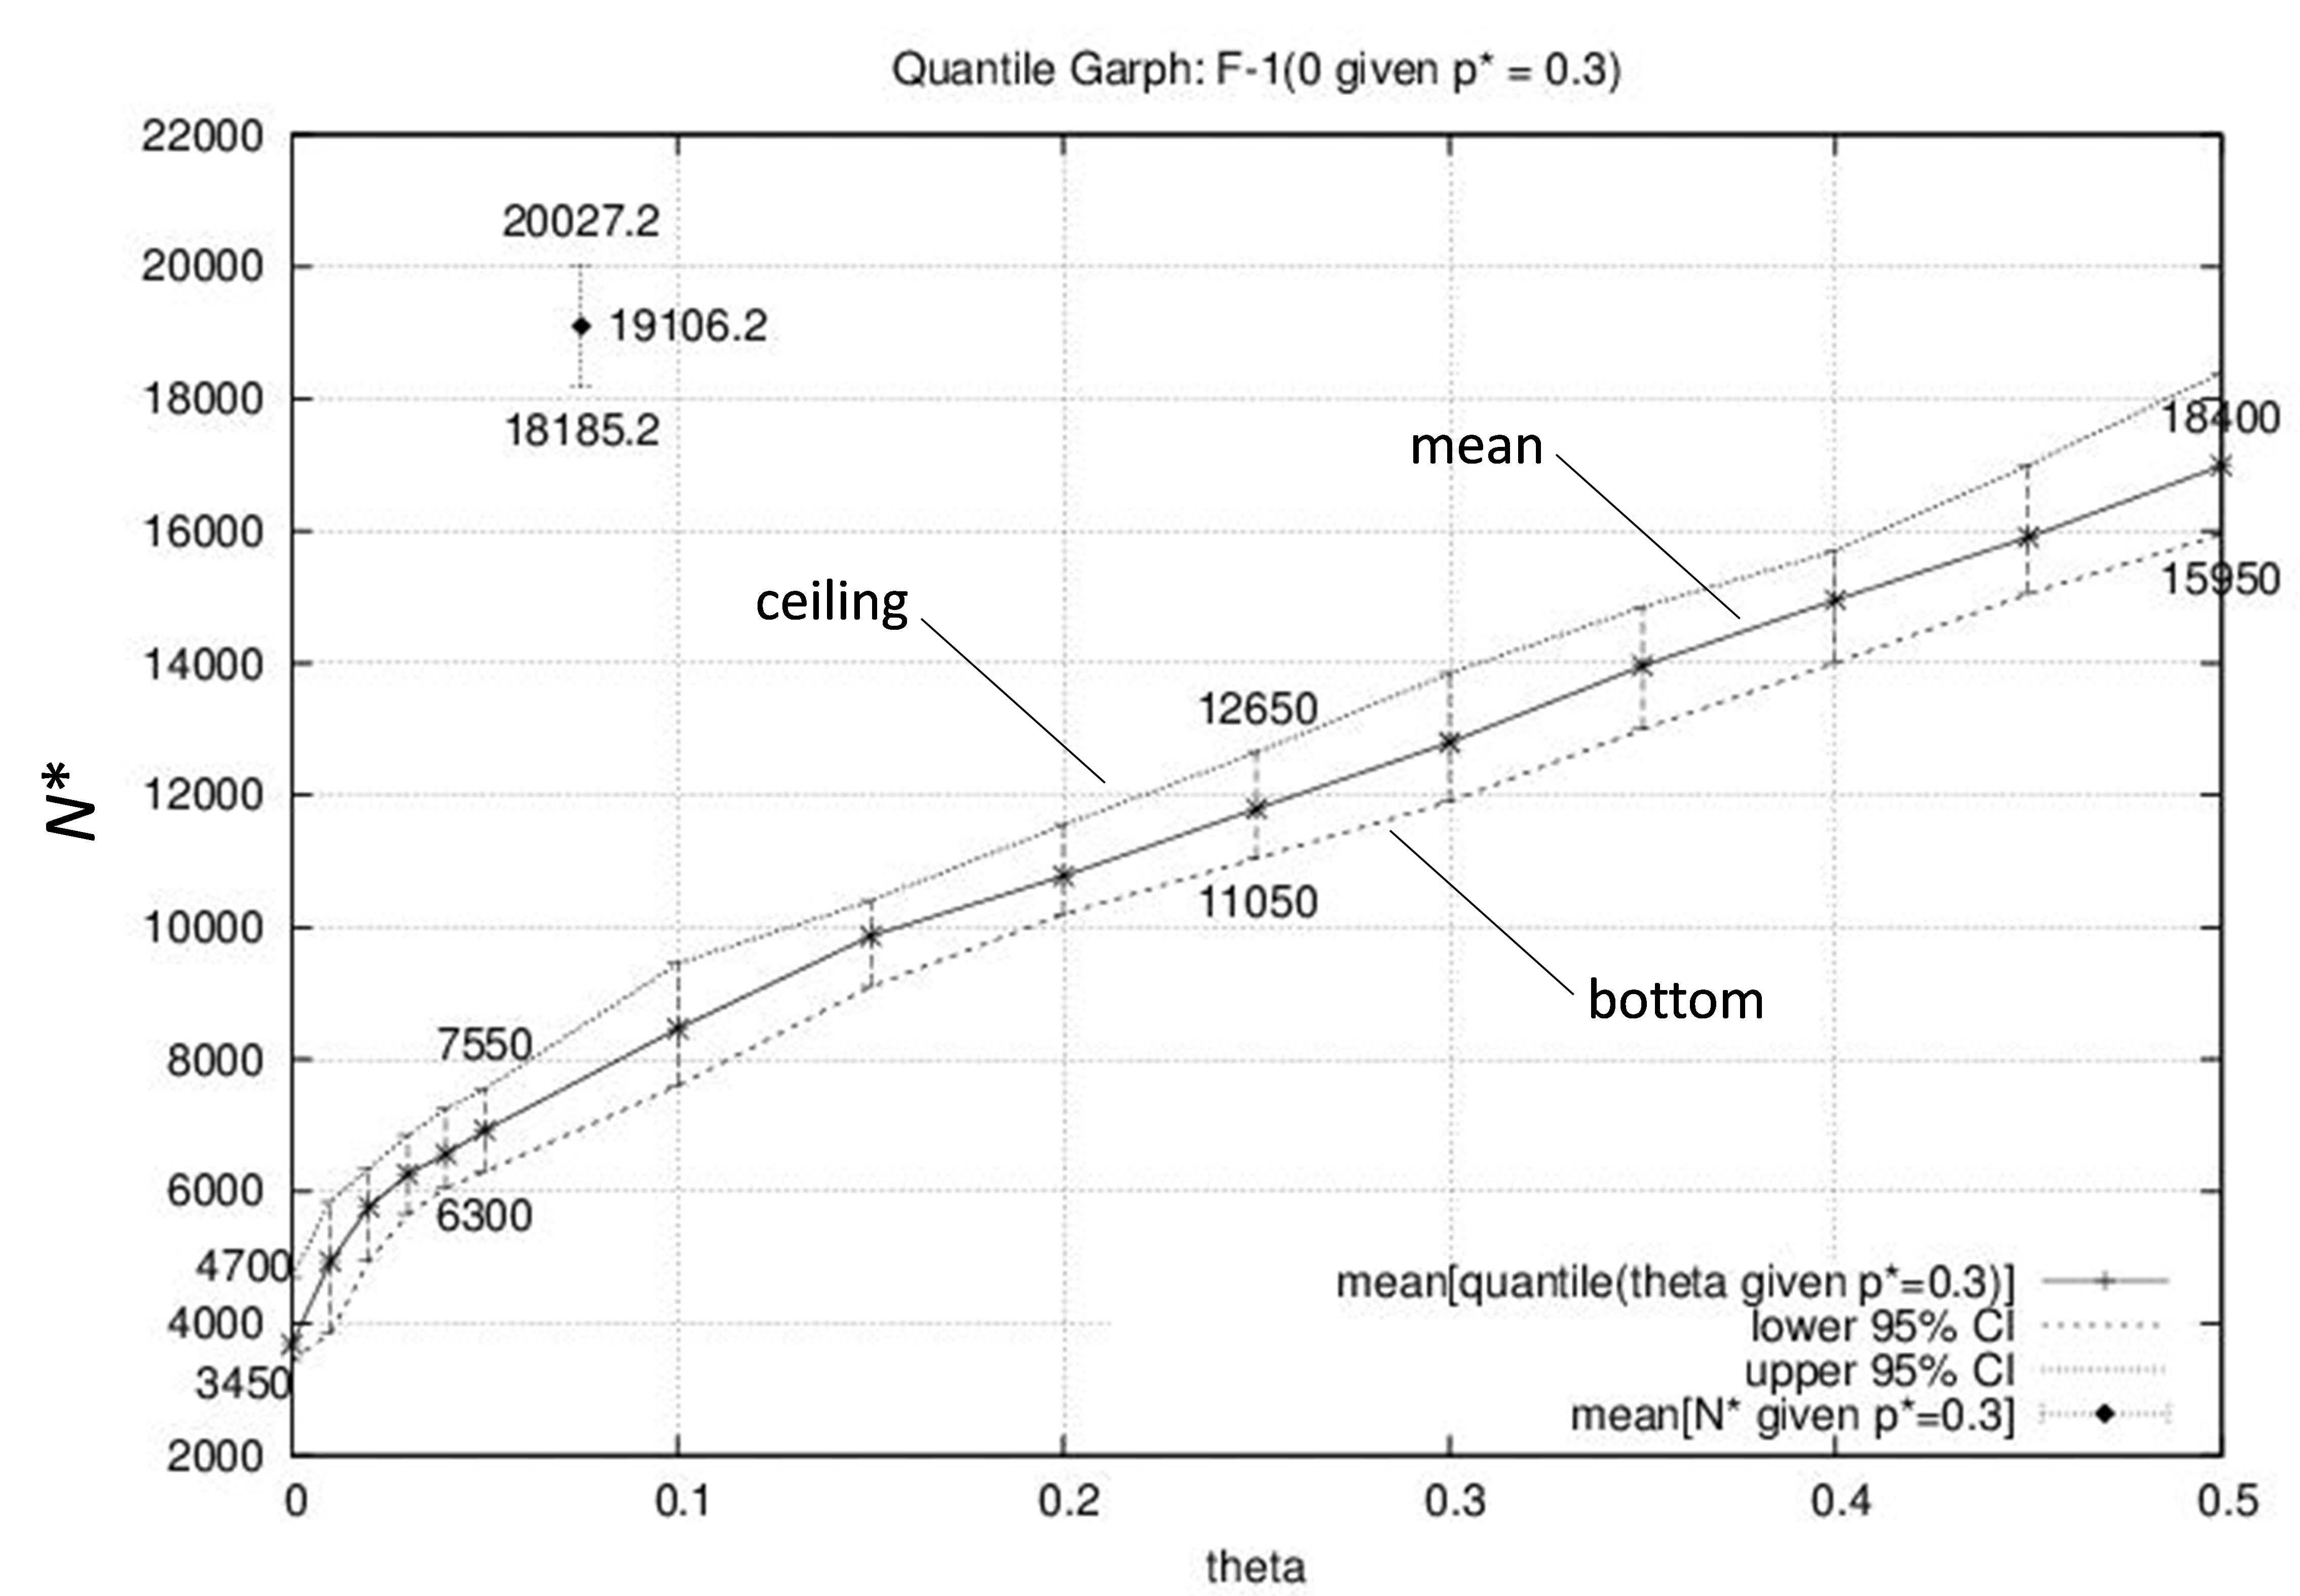
\includegraphics[width=0.9\textwidth]{images/fig6.png}
\end{figure}


\begin{figure}
\centering
\label{fig7}
\caption{$N^*$ for different levels of the probability for $\theta = 0.01$ through $0.50$ an adversary achieves for an accuracy level of $p^* = 0.45$ and $0.50$.}
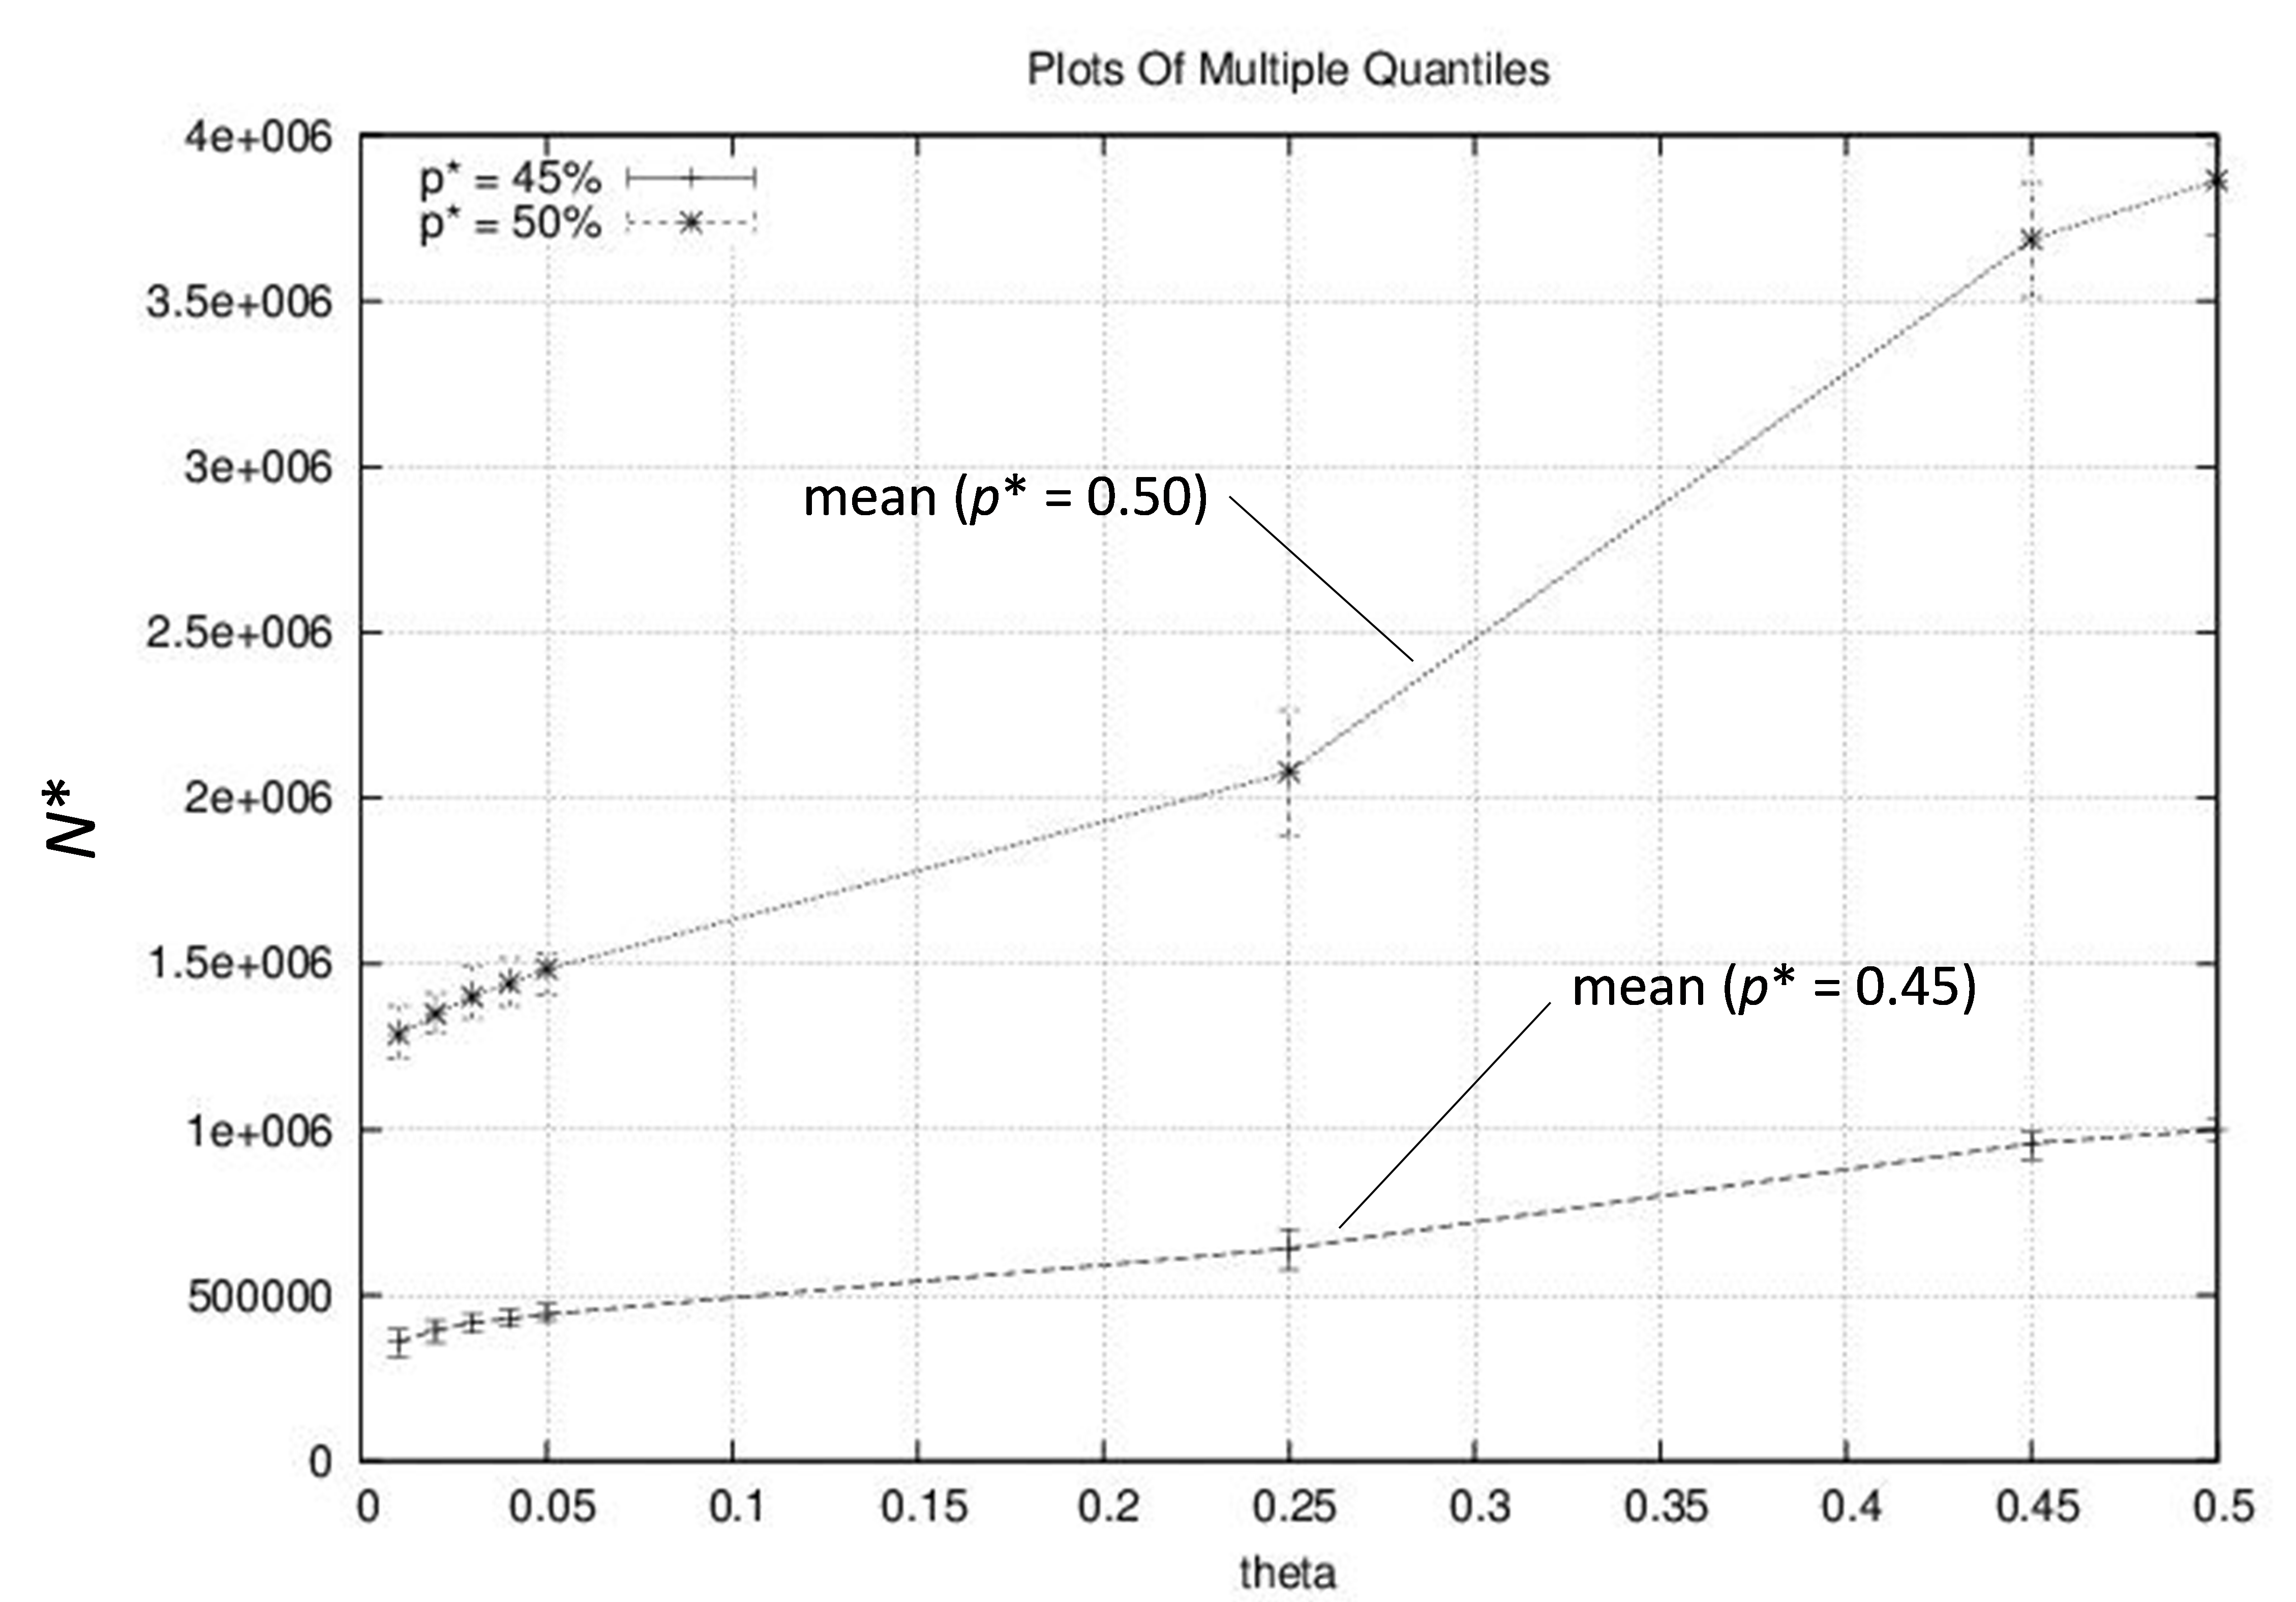
\includegraphics[width=0.9\textwidth]{images/fig7.png}
\end{figure}

\Cref{fig7} shows the $N^*$'s to achieve $p^* = 0.45$ and $0.5$ at the probability of $5\%$ ($\theta = 0.05$). We estimated the mean is around 19,100 observations ($N^* = 19100$) for $p^* = 0.45$.

The followings are the observations from our experiments:

The proposed MAB method calculated the estimated number of encrypted search queries an adversary needs to observe $N^*$ for achieving a given accuracy level, $p^* = 0.30$, at the confidence level of $95\%$ using only $5\%$ of the actual observations ($250/5000$) (\Cref{fig5c}).

For $5\%$ chance that the adversary can read 30\% of what the adversary observed (i.e., $\theta = 0.05$ for $p^* = 0.3$), we estimated that the adversary would need around 6,900 observations ($6900$ encrypted words, $N^* = 6900$). The $95\%$ confidence interval of all the $s$ averages of $m n^*$'s was $[6,300, 7,550]$ encrypted words when $m = 500$ (\Cref{fig6}).

For comparison, for $p^* = 30\%$ accuracy, the estimator $N^*$ estimates the adversary only needs around $5000$ encrypted words to be observed. (Figure 6). For a $\theta = 50\%$ chance of success, the estimator $N^*$ estimates the adversary needs around $17000$ observations for 50\% of success in achieving $p^* = 0.30$ with $m = 500$ (\Cref{fig7}).

For $p^* = 50\%$ accuracy, the estimator $N^*$ predicts the adversary needs a sample size around $360000$ to have a $\theta = 1\%$ chance of success (\Cref{fig7}).

For $p^* = 50\%$ accuracy, the adversary needs around $N^* = 1.3 \times 10^6$ samples (\Cref{fig7}).
\end{document}